\documentclass[11pt]{article}
% =====================================================================
% JEPA Latents Do Not Self-Organize by Timescale
% Style rules for this draft, fixed by the authors:
%   short sentences, active voice, no dashes in prose (ranges use "to"),
%   every number traces to a JSON artifact, every criterion was
%   preregistered before its run, negative results are reported as such.
% Compile: pdflatex main && bibtex main && pdflatex main && pdflatex main
% (or upload the folder to Overleaf).
% =====================================================================
\usepackage[margin=1in]{geometry}
\usepackage{amsmath,amssymb,amsfonts}
\usepackage{graphicx}
\usepackage{booktabs}
\usepackage[numbers,sort&compress]{natbib}
\usepackage[colorlinks=true,linkcolor=blue,citecolor=blue,urlcolor=blue]{hyperref}
\usepackage{microtype}

\title{JEPA Latents Do Not Self-Organize by Timescale:\\
Laws, Diagnosis, and a Minimal Recipe to Force It}
\author{Jiaqi Wang\\ \texttt{jacky777wang@gmail.com}}
\date{October 2026}

\newcommand{\tauc}{\tau}
\newcommand{\term}[1]{\textbf{#1}}

\begin{document}
\maketitle

\begin{abstract}
World model research builds hierarchies to isolate error across timescales.
The field has not checked whether the hierarchy exists.
We measure the timescale organization of JEPA latent spaces and find none.
Six training configurations from two codebases, all small to medium scale, produce a gapless spectrum.
No separation between fast and slow subspaces.
No concentration of slow content.
No levels a planner could iterate.
The failure follows laws.
A decay coefficient cannot be learned from a prediction loss; the loss buys a shrinkage factor, not a decay rate.
The measured dynamics is the least squares solution; every structured family we tested falls short of it.
Coordinate quality sets the ceiling for every dynamics.
A design clock, a measured clock, and a content clock are three different objects, and confusing them caused every defect in our own hierarchy attempt.
The laws point to a minimal recipe: measure the clocks, freeze the measured dynamics, learn only the coordinates.
The recipe buys the best coordinate organization we have measured and one honest boundary: reorganizing coordinates does not extend the horizon a planner can trust.
We deliver the audit protocol, the laws, and the recipe, as instruments for anyone stacking levels on JEPA latents.
\end{abstract}

\section{Introduction}
\label{sec:intro}

A world model that rolls forward one step at a time multiplies its errors.
In our teleoperated PushT data, the slow content of an E$^2$-JEPA latent loses accuracy after 11 steps, while the task needs 22 or more.
Long horizon planning fails before it starts.

The field answers with hierarchy.
Latent world models stack levels with different prediction strides, so that slow levels do not inherit the fast levels' noise
\citep{hjepa,lewm}.
The idea is old and sound: separate timescales, isolate errors.
The JEPA family, trained to predict its own embeddings, carries the wave
\citep{ijepa,vjepa}.

The field skips a question.
Does the hierarchy exist in the representation at all?
The architecture papers measure behavior, not geometry.
Hierarchy in the loss graph is not hierarchy in the latent space.
If the latents carry no timescale structure, then stacking levels on top of them stacks levels on sand.

We measure.
We build an instrument for timescales, audit six trained systems, and find a clean negative result.
The spectrum of latent timescales is gapless everywhere we look.
We then ask why, and the answer condenses into laws.
Finally we ask what forcing hierarchy costs, and the laws dictate a recipe.

Our discipline is preregistration.
Every criterion in this paper was fixed before its run, and the record lives in the released artifact directory with file timestamps.
Thresholds never moved after results arrived.
Three of our own predictions failed, and each failure is reported and used
(Sec.~\ref{sec:phenomenon} and Sec.~\ref{sec:laws}).
The negative results carry most of the information.

The paper contributes four things.
\begin{enumerate}
\item \term{A first report.} The latent timescale spectrum of JEPA family models is gapless, across six configurations from two codebases and four training objectives (Sec.~\ref{sec:phenomenon}).
\item \term{An instrument.} A timescale estimator with four credibility guarantees, calibrated against synthetic signals and external ground truth (Sec.~\ref{sec:instrument}).
\item \term{Laws.} Three quantitative laws and one identity that together explain the failure and constrain every fix (Sec.~\ref{sec:laws}).
\item \term{A minimal recipe.} Measure the clocks, freeze the measured dynamics, learn only the coordinates. The recipe follows from the laws, not from architecture fashion (Sec.~\ref{sec:recipe}).
\end{enumerate}

The paper is a criteria study, not an architecture race.
It answers three questions the race leaves open.
When does a hierarchy exist.
When can it never emerge.
Where must the forcing come from.
Any architecture can use the answers as an acceptance test.

\section{The instrument: measuring a timescale}
\label{sec:instrument}

We need a number before we can have a law.
This section defines the number and proves it can be trusted.

\subsection{The estimator}

Let $x_i(t)$ be one coordinate of a latent, sampled per environment step within an episode.
Its autocorrelation is $C_i(\Delta)$.
The timescale is the truncated autocorrelation integral
\begin{equation}
\tauc_i \;=\; \sum_{\Delta=0}^{k_i} C_i(\Delta),
\label{eq:tau}
\end{equation}
where $k_i$ is the first lag at which $C_i$ turns non-positive.
The truncation rule is the initial positive sequence rule, a classical device from Markov chain diagnostics \citep{geyer92}.
Episodes never share pairs.
The estimator probes the same object that spectral map methods estimate, the relaxation spectrum of the underlying dynamics, from a different angle: the integral of one coordinate's autocorrelation mixes the operator's eigenmodes, each mode contributing with the weight of its share in that coordinate.
A coordinate that is a dense mixture inherits an averaged clock; that averaging is the mechanism behind several results below (Secs.~\ref{sec:credibility} and \ref{sec:threeclocks}).
The estimator is defined for asymptotically stationary coordinates; we state this domain openly, because one important number below (the 437-step contaminant) sits at its edge.

Why this quantity.
A slow feature changes little while a fast feature changes often.
The autocorrelation integral counts how long a feature remembers itself.
The number is in environment steps.
A latent dimension with $\tauc = 100$ remembers itself for about a hundred steps.

\subsection{Four credibility guarantees}
\label{sec:credibility}

An estimator earns trust by failing in public.
Ours carries four guarantees.

\paragraph{Two independent estimators.}
Estimator A integrates autocorrelations of the data (Eq.~\ref{eq:tau}).
Estimator B reads the eigenvalue spectrum of the trained predictor's Jacobian, $\tauc = -1/\ln|\lambda|$.
The two share no code path.
On the E$^2$-JEPA model, B returns a continuous spectrum from 0.14 to 19.6 while A returns 9 for almost every coordinate, with a spread so narrow that adjacent sorted values never differ by more than 3 percent.
Both are right, and the reason is the finding itself.
B reads the dynamics the model learned: many timescales, well separated.
A reads the coordinates the encoder hands to the outside world: the encoder mixes modes densely across coordinates, and dense mixing averages the timescales into one narrow band.
The model learned multiscale dynamics.
The coordinates did not inherit it.

\paragraph{External calibration.}
The LeWM backbone ships seven neutral modes from its integrator, a property of the data pipeline, not of our code.
The \term{participation ratio} of a representation is the squared ratio of its covariance eigenvalue sum to the sum of squared eigenvalues: 1 for a collapsed single direction, $d$ for an isotropic $d$-dimensional code.
Our estimator assigns the seven neutral modes a participation ratio of 6.2, which matches the intrinsic dimension of the PushT observations.
The instrument reads a structure it was never pointed at.

\paragraph{Self exposure.}
An energy-only control collapses its representation to a near constant, with per-dimension std 0.003 and participation ratio 4.6.
The estimator reports a slow $\tauc$ of 15.6 for this junk.
A constant signal remembers itself forever and carries no information.
This exposes the exact domain of the estimator: $\tauc$ is defined only when the representation carries entropy.
The free energy form $F = U - T S$ is not decoration.
The entropy term is the existence condition for the timescale.
Every $\tauc$ in this paper is reported together with a survival guard, $\mathrm{std} \geq 0.01$.

\paragraph{Synthetic calibration.}
We plant AR(1) signals with true timescales 2, 5, 10, 22, and 40 steps.
The estimator returns 2.7, 4.8, 7.2, 10.8, and 12.9 (Fig.~\ref{fig:calib}).
The order is monotone and robust.
Large timescales are compressed by a bounded factor, because a piecewise-constant signal spends its long memory as a nonzero mean, which per-episode demeaning removes.
Absolute numbers in this paper are read with this calibration curve attached.
The calibration also separates the instrument's two uses.
For pure AR(1) signals at large $\tauc$, the integral reads low; the ordering, which is what the audit and the laws use, stays strict.
The content clock check of Sec.~\ref{sec:threeclocks} uses a second, independent estimator (a windowed fit of a rollout readout), and its agreement with the task-side ground truth is a cross-validation between two instruments, not a restatement of the synthetic curve.

\begin{figure}[t]
\centering
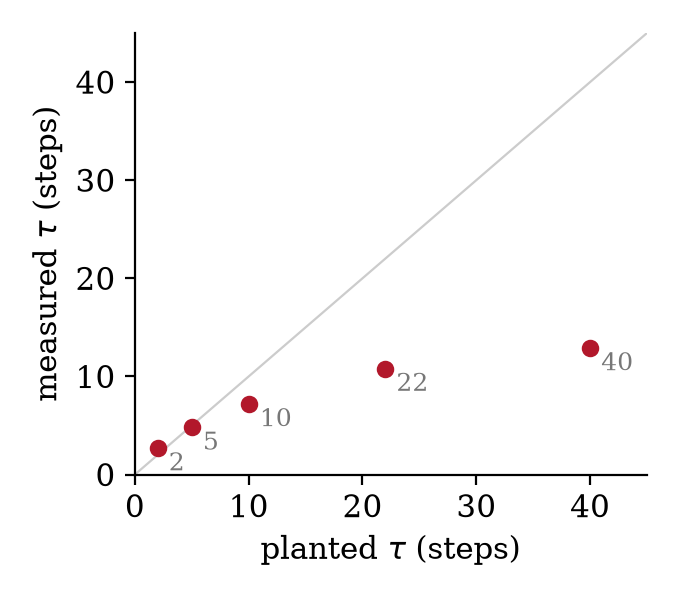
\includegraphics[width=0.42\linewidth]{figs/calibration.png}
\caption{Synthetic calibration of the estimator. Planted AR(1) timescales against measured ones. The order is strict; large planted values are compressed by a bounded factor (per-episode demeaning absorbs piecewise-constant memory).}
\label{fig:calib}
\end{figure}

\subsection{Content ground truth}
\label{sec:groundtruth}

Latent timescales need content timescales to be judged against.
We measure the task directly.
PushT teleoperation data segments itself: block strokes are visible as displacement runs.
Stroke segmentation needs no labeler.
From the segmentation, the block pose carries $\tauc = 22.7$, the agent pose $\tauc = 13.5$, and the velocity layer $\tauc \approx 2$.
Block time splits evenly between strokes and dwells, with medians of 17 and 16 steps, three strokes per episode.
These numbers are ground truth for every content claim in this paper.
A second, independent estimator reproduces them to within one percent (Sec.~\ref{sec:threeclocks}, the content clock check), which is the instrument's strongest external cross-validation.

\section{The phenomenon: the gapless spectrum}
\label{sec:phenomenon}

\subsection{Notation}
\label{sec:notation}

The audit needs six terms, and we define them once here.
A \term{probe} $\mathrm{R}^2$ is the coefficient of determination of a linear ridge readout from latent coordinates to a content label, fit on training episodes and scored on validation episodes.
A \term{band} or \term{block} is a group of 16 latent coordinates treated as one unit by the organization layer.
\term{Banding} is the training pressure that pushes each band's cross-covariance decay toward a target timescale.
E$^2$-JEPA is our JEPA variant trained with a free energy objective, an energy term plus an entropy term.
The \term{smoothing end} of the design space uses entropy regularization without variance collapse protection; its coordinates smear.
The \term{compressing end} uses variance-covariance regularization in the VICReg style \citep{vicreg}; its coordinates homogenize.
The \term{least squares operator} is the free per-block solution, the fourth operator family we evaluated and the one the laws keep.
A \term{null} is the same pipeline run on time-shuffled data, which destroys dynamics and keeps marginals.
The \term{content trust horizon} is how far a rollout of the model keeps a content readout above a fixed accuracy bar.
The quantity $\epsilon^*$ in H4 is the residual cross-block coupling after the best partition of the coordinates into $K$ blocks, normalized by the same partition applied to a time-shuffled copy: 1 means the partition explains nothing, 0 means perfect blocks.

\subsection{Falsifiable criteria for hierarchy}

Hierarchy is a geometric claim about the latent space, so it gets geometric criteria.
Table~\ref{tab:hstandard} states five.
Each is falsifiable, each has a threshold fixed in advance, and each guards the next.

\begin{table}[t]
\centering
\caption{The H-standard. A representation is hierarchical when all five hold. Thresholds were fixed before any audit run. H1 and H2 are decided by the spectrum and the top-8 column: a gapless spectrum fails H1, and if the slowest-sorted dimensions carry no more slow content than random, H2 fails with them.}
\label{tab:hstandard}
\begin{tabular}{llp{7.2cm}}
\toprule
Criterion & Threshold & Meaning \\
\midrule
H1 separation & spectral gap & the timescale spectrum has a gap between clusters \\
H2 alignment & correlation & slow coordinates carry the slow content \\
H3a concentration & top-8 $\geq$ 0.8 $\times$ full & a small subset of dimensions suffices for the slow content \\
H4 block structure & $\epsilon^* \leq 0.5 \times$ null & coordinates split into blocks with weak cross coupling \\
H5 assembly & err(16) $\leq$ 0.5 & the slow block iterates alone 16 steps without diverging \\
survival guard & std $\geq$ 0.01 & the representation has not collapsed \\
\bottomrule
\end{tabular}
\end{table}

A method needs a positive control before it needs a result.
We plant a block structure in synthetic data and ask the H4 test to find it.
It finds the planted blocks at $\epsilon^* / \mathrm{null} = 0.049$, near-perfect recovery.
We plant iid coupling instead.
The test rejects it at 0.897.
The instrument passes 13 of 13 self checks.
The negative results below are therefore measurements, not artifacts.

\subsection{The audit}

We audit six trained systems.
Four are ours: E$^2$-JEPA, a TV-regularized variant, a plain JEPA, and an energy-only control.
All four train on the same teleoperated PushT data, in our codebase.
Two are external backbones from the stable-worldmodel platform \citep{swm}: the LeWM world model, audited on the same data, and an H-JEPA backbone, whose spectrum we measure directly in Sec.~\ref{sec:handplaced}
\citep{lewm,hjepa}.
Two codebases, six systems.
The setup is small and we say so.
The teleoperated PushT data runs about 200 episodes per training arm; the AntMaze offline data runs 310 episodes.
LeWM carries about 15 million parameters \citep{lewm}; our four self-trained systems are smaller.
The organization layer trains 6000 steps on a 128-dimensional readout of each frozen backbone.
The scale is a limitation we own (Sec.~\ref{sec:discussion}); the protocol is what transfers.

\begin{table}[t]
\centering
\caption{The audit. Five systems against the H-standard, measured on the same teleoperated PushT data (collected by the authors on a push-T task). The H-JEPA backbone enters the structural audit in Sec.~\ref{sec:handplaced}, where its spectrum is measured directly. H3a reports the top-8 slow-content recovery as a fraction of the full-128 recovery; the threshold is 0.8. The best system (LeWM) reaches 0.64; none passes. H4 shows the ratio $\epsilon^* / \mathrm{null}$ over $K = 2$ to 5 blocks; the threshold is 0.5. The LeWM $h^*$ entry comes from the macro-5 natural experiment (Sec.~\ref{sec:phenomenon}); its own stride-1 H5 was not measured. Every system fails every structural criterion.}
\label{tab:audit}
\begin{tabular}{lccc}
\toprule
System & H3a top-8 / full & H4 $\epsilon^*$ ratio & H5 horizon $h^*$ \\
\midrule
E$^2$-JEPA & 0.17 / 0.76 = 0.22 & 0.96 to 0.98 & 11 \\
Plain JEPA & 0.28 / 0.75 = 0.37 & 0.87 to 0.93 & 15 \\
TV variant & 0.32 / 0.76 = 0.42 & 0.86 to 0.94 & 18 \\
Energy-only & collapsed & below guard & 1 \\
LeWM & 0.37 / 0.58 = 0.64 & 0.82 to 0.89 & 25 (macro head) \\
\bottomrule
\end{tabular}
\end{table}

\begin{figure}[t]
\centering
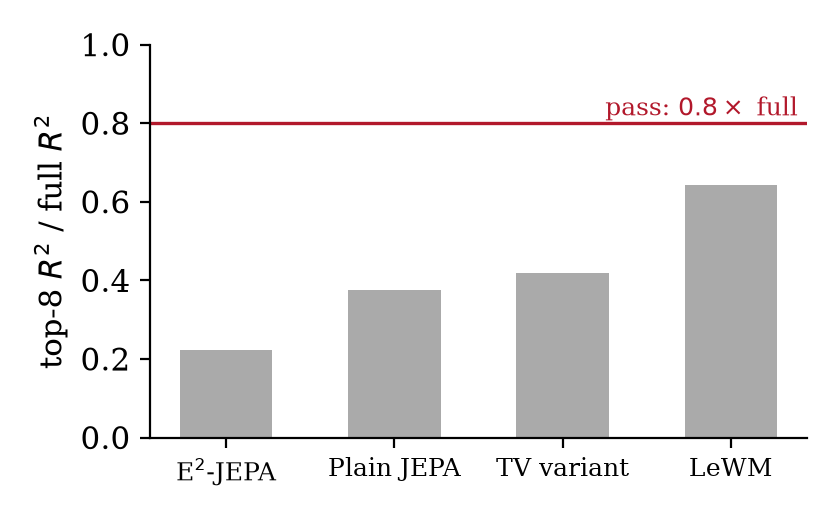
\includegraphics[width=0.55\linewidth]{figs/audit_bars.png}
\caption{The H3a column of Table~\ref{tab:audit}. Top-8 recovery as a fraction of full, against the 0.8 threshold. The energy-only control is off scale (collapsed).}
\label{fig:auditbars}
\end{figure}

Table~\ref{tab:audit} carries the paper's first finding.
The H3a column reports how much of the slow content a top-8 subset of the $\tauc$-sorted coordinates recovers, as a fraction of what all 128 dimensions recover.
The smoothing end recovers little.
E$^2$-JEPA and plain JEPA reach 0.22 and 0.37 of full, against a passing mark of 0.8, and a random subset of the same size reaches 0.21 and 0.35 on the same systems, so the $\tauc$-sorted top-8 holds no more slow content than chance.
The TV variant reaches 0.42, against a random baseline of 0.30.
The compressing end (LeWM) does best at 0.64, against a random baseline of 0.51, and its coordinates are so homogenized that no block survives: its $\epsilon^*$ ratio is 0.82 at best, against a passing threshold of 0.5.
H4 fails everywhere, with $\epsilon^*$ ratios from 0.82 to 0.98 across the systems above the guard and all block counts.
The latents have no blocks to build a hierarchy from.
The energy-only control fails first: it collapses (per-dimension std 0.003), fails the survival guard, and its slow projection diverges from the first step.

The gapless spectrum itself is worth a sentence of numbers.
Figure~\ref{fig:taus} shows the three self-trained arms that pass the survival guard.
Across the self-trained arms, adjacent sorted timescales never differ by more than 8 percent.
A representation organized by timescale would show clusters, with gaps of at least 15 percent between them.
Ours shows a continuum.

\begin{figure}[t]
\centering
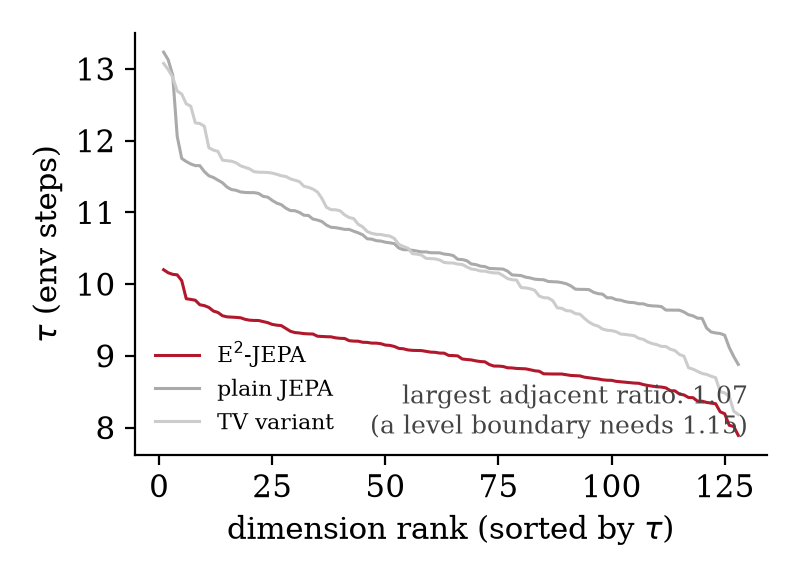
\includegraphics[width=0.55\linewidth]{figs/tau_sorted.png}
\caption{The gapless spectrum. Sorted per-dimension timescales of the self-trained arms that pass the survival guard. The curves are continua with no cluster and no gap: the largest ratio between adjacent sorted timescales is 1.07, and a level boundary needs 1.15. The energy-only control fails the guard and has no defined timescale.}
\label{fig:taus}
\end{figure}

\subsection{Two natural experiments}

Two measurements in the external systems cut deeper than the audit table.

\paragraph{Stride buys tracking, not structure.}
The LeWM release ships a macro-action head trained at stride 5.
It is the field's hierarchy in miniature: one level, longer steps.
The macro head reaches $h^* = 25$, clearly past the stride-1 arms at 11 to 18.
Longer strides do improve single horizon tracking.
But the improvement does not deposit into the coordinates.
H4 still fails, and a slow projection of the latents dies at $h = 4$.
The stride bought a longer lever.
It did not buy a place to stand.

\paragraph{Error compounding dominates information.}
The same LeWM latents reach error 0.28 at 20 steps when asked directly, but error 0.70 when iterated.
The E$^2$-JEPA shows the same signature, error 0.87 direct against 1.18 iterated at 16 steps.
The slow content is predictable.
The iteration destroys it.
This is the engineering argument for hierarchy in one line, and also the reason a fake hierarchy fails: iteration reads the levels you actually have, not the levels you drew.

\subsection{Hand placed hierarchy is not hierarchy}
\label{sec:handplaced}

H-JEPA stacks levels with pooled strides of 5, 10, and 20.
We measure what the stacking does to the operator spectrum.
Each level spans two orders of magnitude of continuous timescales.
The largest gap between adjacent modes is 1.37, and a ladder needs every gap clear, not one: the rest sit at or below the noise between neighbors.
A spectrum with one large gap among continuous stretches is a single split, not a ladder of levels.
Per level, the median timescale drifts only 1.5 to 1.7 times.
An architecture can have levels the way a building can have painted doors: the paint is real, the rooms are not.

The observation generalizes.
A high level ignoring moving obstacles, as H-JEPA reports on AntMaze, is functional division of labor, not structural hierarchy.
Function can come from the task's own forcing (Sec.~\ref{sec:mechanism}).
Structure is a property of the spectrum.
The two can diverge, and when they diverge, planning inherits the structure, not the function.
Sec.~\ref{sec:mechanism} separates the two and Sec.~\ref{sec:laws} shows what each is worth.

\section{Laws}
\label{sec:laws}

The audit says hierarchy does not emerge.
This section says why, in the form of laws.
Each law survived the falsification attempts we preregistered against it.
We tested each law on at least three datasets: PushT, AntMaze with a LeWM backbone, and AntMaze with an H-JEPA backbone.

\subsection{L1. A clock is measured, not learned}
\label{sec:l1}

A prediction loss contains a multiplicative decay coefficient $\rho$ per band.
It is tempting to make $\rho$ learnable and let the loss discover each band's timescale.
We ran the experiment with the banding target frozen and the rest of training unchanged: the encoder still learned, only $\rho$ joined the parameter set.
The loss dropped by an order of magnitude, from 0.104, 0.343, and 0.246 to 0.0001, 0.029, and 0.028 across the three datasets.
The banding term, whose reference is a frozen target, did not move.
The learned $\rho$ ran to the extremes.
On real data the learned values hit the clamp at $\rho = 0.999999$ on five of eight bands (PushT) and eight of eight on both AntMaze backbones, while the slowest band's own cross-covariance on AntMaze fell from 0.96 at lag 1 to 0.22 at lag 32.
The learned clock was not the coordinate's clock.
The two differed by an order of magnitude.

The mechanism is algebra, not anecdote, and its scope matters.
Under a relative squared error, the optimal multiplicative coefficient equals the shrinkage of the predictable part of the target, not the decay rate of the data.
A high signal band wants the coefficient at 1.
A noise band wants it near 0.
The loss cannot tell slow decay from unpredictability, because it never sees the decay without the noise.
Prediction therefore buys persistence, and persistence is what a collapsed hierarchy is made of.
The claim is bounded: it covers a scalar multiplicative coefficient under a relative squared error, which is what a per-band decay term is.
It does not forbid every conceivable way of learning a clock, and the schedule result of Sec.~\ref{sec:taskshape} shows one thing that does order content.
The experiment closes with the content clock: the learned clock made the slow content appear 2.0 to 3.2 times slower than ground truth, while the measured clock sat within 1 percent.
Clocks are measured.

\subsection{L2. The measured dynamics is the least squares solution}
\label{sec:l2}

If clocks cannot be learned, what should the dynamics be?
We compared operator families on the same coordinates, with the same split, at every horizon.
The free per-band least squares operator beats the identity map by 18 to 30 percent on pooled error.
It beats every structured family we tried.
Diagonal decay, conformal decay with rotation, rank-k truncations: all fall short, and the rank-k families fall further as k shrinks.
The family budget is small.
Lifting the conformal family to a free 16 by 16 block buys only 0.004 to 0.033 of validation error across datasets.

The law survived the strongest test we could design for it.
We replaced the learnable dynamics inside training with the frozen least squares solution, fitted once on the initial coordinates, and retrained end to end.
Zero learnable dynamics parameters.
The criteria that passed before still passed.
The prediction error did not collapse.
Training inside a frozen measurement is not a limitation.
It is the measurement, taken seriously.

\subsection{L3. Coordinate quality is the ceiling}
\label{sec:l3}

Law L2 says any dynamics lives or dies with its coordinates.
The experiment that proves it is our own worst result.
When the clock was learnable (the L1 experiment), the coordinates degraded.
The same operator, the same data, the same split, degraded 1.8, 3.7, and 4.2 times on the three datasets relative to the frozen-clock run.
No dynamics in our study recovered what bad coordinates lost, and the least squares operator lost the least.
Dynamics is a lens.
The coordinates are the specimen.

\subsection{The placement law}
\label{sec:placement}

Content settles at its own timescale, when given a place to settle.
In the AntMaze decompositions, pose content occupies the slowest band with probe $\mathrm{R}^2$ of 0.818 to 0.857, and velocity content peaks in the fastest band at 0.215 to 0.312.
The velocity layer's ground truth is $\tauc \approx 2$, and the fastest band's clock is $\tauc \approx 3$.
The slowest band's monopoly on pose is not a failure of allocation.
It is the correct equilibrium for a persistent variable.
We preregistered the opposite hypothesis, winner-take-all allocation, and the data falsified us.
The failure mode that remains is not misallocation.
It is the absence of coordinates where fast content is linearly readable at all.

\subsection{The three clock identity}
\label{sec:threeclocks}

The deepest defect in hierarchical world models is a category error, so we state it as an identity.
Three clocks hide inside every design.
The \term{design clock} is what the architecture declares: this band holds timescale 102.
The \term{measured clock} is what the frozen least squares operator of Sec.~\ref{sec:l2} returns: spectral radius 0.9977, timescale 437.
The \term{content clock} is what the content itself keeps: the AntMaze position variable relaxes in 9 steps.
The design clock overestimates the content clock by 2.5 to 11 times across our three datasets.
The measured clock overestimates it further, because persistent data pushes least squares eigenvalues toward the unit circle.

We found the identity the hard way.
Our own banding target encoded the SFA modulus, a design clock.
The trained bands stretched toward it, and we measured whether the stretched bands carried stretched content.
They did not.
The content trust horizon ran 2.9 to 7.5 times faster than the band it lived in.
The stretch was hollow.
We then replaced the banding target with the content clock and retrained.
The organization improved everywhere: content segregation reached its best values in the project's history, 0.358, 0.536, and 0.507.
The content trust horizon did not move.
It stayed at 40.26 on the H-JEPA backbone, the same number, because the rollout dynamics was frozen at the measured operator and the measured operator carries a 437-step contaminant.
Banding is an organization force, not a dynamics force.
L1 and L2 predicted this before the run, and the run obliged.

\subsection{The dimensionless clock law}
\label{sec:clocklaw}

One measurement certifies the whole instrument.
Evolve each band with its fitted operator for $h$ steps and compare with the truth.
The error tracks $\sqrt{1 - \rho_k^{2h}}$ per band, with maximum ratio 1.53 across all bands and datasets.
Rescale time by the band's own clock, and all bands collapse onto one curve (Fig.~\ref{fig:collapse}).
At $h = 2\tauc$ the spread across bands is 0.006 to 0.068.
The ladder is not a descriptive statistic.
It is each band's physical time, the same way a half-life is.

\begin{figure}[t]
\centering
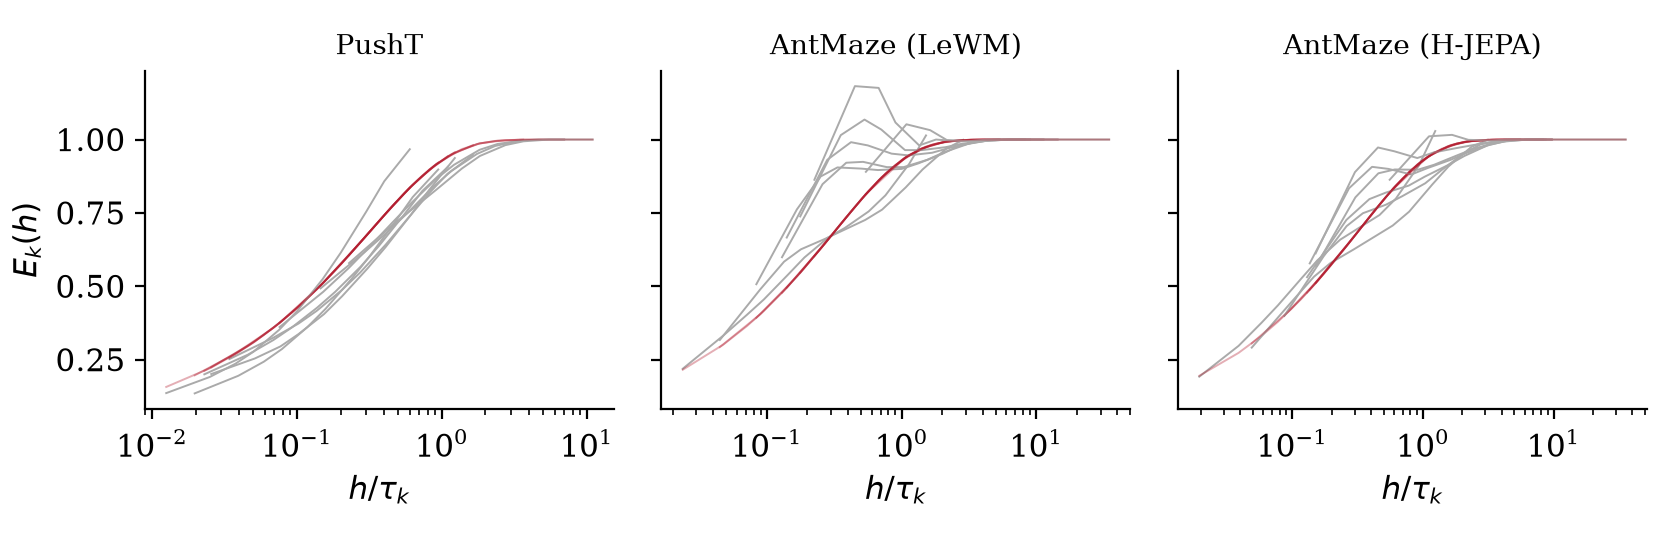
\includegraphics[width=0.9\linewidth]{figs/clock_collapse.png}
\caption{The dimensionless clock law. Rollout error of each band against horizon rescaled by the band's own $\tauc$. Grey: measured curves for all eight bands. Red: the predicted form $\sqrt{1 - \rho_k^{2h}}$. The bands collapse onto one curve in $h/\tauc$, which makes the ladder a physical clock rather than a summary statistic.}
\label{fig:collapse}
\end{figure}

One criterion retired under this law.
A pooled displacement $\mathrm{R}^2$ is a rapidity weighted average, with weights proportional to $1/\tauc$.
An ideal ladder tuned to its own optimum cannot exceed 0.21 under the weights our data produce.
A threshold of 0.37 was unreachable by any honest multiscale representation.
We retired the criterion, and we report the algebra that retired it.
A criterion that survives on a misreading is a liability, not an asset.

\subsection{What the laws forbid, in one paragraph}

No marginal regularizer can force timescale organization, because marginals cannot see joint distributions; the zero loss solution that ignores the joint exists for every one we tested.
Prediction loss cannot teach clocks (L1), so hierarchies that learn their strides are learning shrinkage.
Structure does not deposit from stride schedules, because function is not geometry (Sec.~\ref{sec:handplaced}).
And any fix that confuses the three clocks will purchase organization it cannot spend on content.
What the laws leave open is narrower, and that narrow opening is the recipe.

\section{Why hierarchy does not emerge: the two pathways}
\label{sec:mechanism}

The audit leaves a question.
Self-organized hierarchy is absent, so something must prevent it.
We enumerate the forces that could couple content to timescale, close all but one by experiment, and find the survivor is a property of the task, not of the loss.

\subsection{Enumerating the forces}

Take a JEPA trained without content labels.
Ask where the gradient could learn that some content is slow and some is fast.
The architecture sets the terrain, but terrain does not give direction.
The data decides frame granularity, and content of different speeds shares the same frames.
An independent regularizer cannot break the tie, because it is blind to which content it touches: permuting content leaves the regularizer unchanged.
Explicit supervision is outside the definition of spontaneous organization.
Two pathways remain.
The loss could act through the \term{rate} of representation change, the entropy budget.
Or the loss could act through the \term{shape of the task}, the prediction targets themselves.
Call them the rate pathway and the task shape pathway.

\subsection{The rate pathway closes by experiment}
\label{sec:rate}

The rate pathway says: give the representation more entropy budget, and organization will grow.
We tested it with a hundred-fold sweep of the entropy temperature, from $t_{\max} = 0.03$ to $t_{\max} = 3.0$, one model per point.
The prediction of the rate pathway is monotone: more budget, more slow content, more order.
The data said no.
The block probe fell from 0.825 to 0.730.
The agent probe stayed flat at 0.31 to 0.35.
The participation ratio rose from 79 to 119, which means the budget spread the variance across more dimensions.
The budget bought dimensions.
It did not buy organization.
We registered the prediction, the data falsified it, and the record stands.

The sweep left one clue that later became a law of its own.
The information axis of the sweep was not timescale.
It was action determinism.
Agent content is largely a function of the action stream, and the prediction loss has no reason to store what the actions already determine.
A control measurement confirms the split: under a random-action policy the LeWM backbone carries the agent at probe 0.69, while our action-conditioned data carries it at 0.35.
The loss keeps exactly the content that the action stream does not decide.
Timescale rides along, and is not the cause.

\subsection{The temperature pathway closes by experiment}
\label{sec:temperature}

A temperature vector can act on the banding directly: cool the slow bands, heat the fast ones.
We built the mechanism and preregistered three criteria: band separation in the measured spectrum, content placement against the band it belongs to, and content survival under the guard.
All three failed.
We summarize the outcome rather than the distances, and we say why: the criteria failed below the guard, and the exact distance to a failed threshold is not the finding.
The finding is the asymmetry.
Every directional signal came out correct: temperature raised the survival of slow content in the slow bands and never pushed content into the wrong band.
Temperature decides what \emph{survives} in the representation.
It does not decide where content \emph{settles}.
Survival has a thermostat.
Placement does not.

\subsection{The task shape pathway survives}
\label{sec:taskshape}

The task shape pathway says: predict the same latent at several strides, and the fast content will be evicted from the coarse levels, because it is unpredictable there.
We built the controlled version, three blocks with strides 5, 2, and 1, against a single-stride control with identical budget.
The $\tauc$ ladder appeared: 14.0, 12.4, and 11.8 against a control at 1.01.
To our knowledge this is the first controlled demonstration, within the JEPA family, that a prediction schedule alone orders latent timescales.
It is also small, about a factor of 1.2 across the levels, and it leaves open the question of scale, which Sec.~\ref{sec:recipe} attacks.
The result does not conflict with the macro-head finding of Sec.~\ref{sec:phenomenon}: the controlled layer here imposes band structure explicitly, while the macro head imposes none.

\subsection{The data decides feasibility, in advance}
\label{sec:feasibility}

The task shape pathway needs raw material.
If the data itself has no separation between fast and slow dynamics, no forcing can carve it.
The SFA ladder of the data measures the raw material before any training.
AntMaze has strong separation: its ladder has no mode faster than $\tauc = 3$, and spans up to 102.
PushT is weak: its ladder spans 0.48 to 56.7 with no gap.
AntMaze is the standard offline navigation benchmark \citep{d4rl}, encoded through the stable-worldmodel platform \citep{swm}.
Before running any organization layer, we registered the prediction: AntMaze will support it, PushT will resist it.
The prediction held (Sec.~\ref{sec:recipe}).
We flag this as the paper's own acceptance test of the criteria approach: the measurement called the outcome before the run.

\subsection{Concordance with theory}
\label{sec:concordance}

H-JEPA's own analysis proves that any regularizer looking only at marginal distributions cannot exclude a zero-loss solution that encodes only the static background \citep{hjepa}.
Our rate sweep is, to our knowledge, the first measurement-level confirmation of that theorem.
The theorem also reads our audit table.
The obstacle-ignoring behavior that H-JEPA reports at its high level is the signature of that degenerate solution family: static background, no moving obstacle, planning-relevant content optional.
Function is real there, and we do not dispute it.
Structure is absent, and the spectrum says so.
The distinction matters downstream.
A planner inherits the structure, and iteration reads the levels you have, not the levels you drew (Sec.~\ref{sec:handplaced}).

\section{The minimal recipe: measure, then learn}
\label{sec:recipe}

The laws of Sec.~\ref{sec:laws} and the one surviving pathway of Sec.~\ref{sec:mechanism} dictate a recipe.
We state the recipe, report its record across three backbones, and show its boundary in the same breath.

The recipe is judged by four criteria, fixed before the first run of the organization layer.
\begin{itemize}
\item \term{C2 segregation:} slow content probes in the two slowest bands minus fast content probes in the two fastest; threshold 0.3.
\item \term{C3 band placement:} the measured band medians must match the ladder, with every adjacent gap at least $1.15 \times$ and every placement within $1.5 \times$ of its target.
\item \term{C4 assembly:} the 20-step rollout error of the layer's frozen dynamics must stay within $1.25 \times$ of a data-fitted DMD on the same coordinates.
\item \term{C1 (retired):} pooled displacement linearity, retired under the weighted average theorem (Sec.~\ref{sec:clocklaw}).
\end{itemize}

\subsection{The recipe}

The organization layer is a post-training adapter.
It takes a frozen JEPA backbone and reshapes a 128-dimensional readout of its latent into 8 blocks of 16, under a free energy objective.
The steps follow from the laws.

\begin{enumerate}
\item \term{Measure the clocks.} Slow feature analysis and DMD on the frozen latents give a ladder of modal timescales \citep{sfa,dmd}. The measured ladder, not a designer's wish, is the skeleton (L1).
\item \term{Span the phase space.} The scaffold augments the 64 slowest directions with 64 increment-PCA directions. A dictionary of observables must contain the near-invariant subspace, and positions alone do not: the dynamics of a second-order system live on the tangent space too \citep{koopman_edmd}. The repair restores the linear content of the AntMaze LeWM backbone 11-fold (0.027 to 0.315).
\item \term{Freeze the measured dynamics.} The prediction operator is the per-block least squares solution, fitted once on the initial coordinates and frozen (L2). Training carries zero learnable dynamics parameters.
\item \term{Band against the content clock.} The banding target is the timescale the content itself keeps, measured from the data by the estimator of Sec.~\ref{sec:instrument} (the three-clock identity).
\item \term{Learn only the coordinates.} The free energy $F = U - T S$ reshapes the coordinates inside the frozen measurement. $U$ is the relative prediction error under the frozen operator, $S$ is the log-determinant entropy of the band covariances, $T$ follows a cooling schedule, and scale anchors hold each dimension's variance near one so the entropy cannot spend itself on overall scale. The entropy term is the existence condition for the timescale (Sec.~\ref{sec:credibility}).
\end{enumerate}

\subsection{The design history, compressed}
\label{sec:history}

The recipe was not designed.
It was excavated, and the failed layers are part of the result.
A fixed-band single-rate layer produced nothing, and the Ising model explains why: a mean-field coupling without topology cannot form blocks.
A phase-conditioned layer ran into the same wall.
The first $\tauc$ ordering came from multi-rate prediction alone (Sec.~\ref{sec:taskshape}).
The measure-then-learn design then appeared: close-form scaffold, free energy on top, and preregistered criteria C1 to C4 to judge it.
Every step after that was a measurement specifying the next move.
The declared clock had to be the measured clock.
The scaffold had to span the tangent space.
The dynamics had to be the least squares solution.
The banding had to encode the content clock.
Each correction was forced by a number, not by taste.

\subsection{The record across three backbones}
\label{sec:record}

Table~\ref{tab:recipe} reports the final configuration: frozen least squares dynamics, content-calibrated banding, 6000 training steps.
A word on the ruler.
The audit uses the H-standard because the audit asks what emerges without structure.
The recipe imposes structure by design, so the honest questions change: does the imposed structure carry the content (C2), does it separate cleanly (C3), does it iterate (C4).
H1 and H3a are criteria for self-organization; the recipe is not self-organization and does not claim their mantle.
The criteria C2 to C4 are the survivors of the family; C1 retired under the weighted average theorem (Sec.~\ref{sec:clocklaw}).
The positive control, run under the measured-ladder protocol (on the synthetic system the planted content clock and the measured ladder coincide), passes: on a planted 8-band system the layer recovers the full geometric ladder at 4 of 4 criteria, with medians 0.95 to 96.5 against a planted 1 to 128.
The null protocol holds: with shuffled time, the segregation excess over the null stays at 0.19 to 0.21 on all three datasets.

\begin{table}[t]
\centering
\caption{The recipe's record, final configuration (frozen LS dynamics, content-calibrated banding). Segregation C2: slow content probes in the slow blocks minus fast content. Assembly C4: 20-step rollout error of the frozen dynamics against a data-fitted DMD on the same coordinates, threshold $1.25 \times$. The placement column reports the slowest band's median against its ladder target.}
\label{tab:recipe}
\begin{tabular}{lcccc}
\toprule
Backbone & C2 seg & C4 err ratio & slow-band placement & $\Delta$seg (null) \\
\midrule
PushT (LeWM) & 0.358 & 0.94 & noise floor & 0.200 \\
AntMaze (LeWM) & 0.536 & 0.98 & 1.9$\times$ stretched & 0.213 \\
AntMaze (H-JEPA) & 0.507 & 0.99 & 1.9$\times$ stretched & 0.194 \\
\bottomrule
\end{tabular}
\end{table}

Three readings of the table.

\paragraph{Segregation is real and best in class.}
Content separation reaches its highest values of the entire project on all three backbones, 0.358, 0.536, and 0.507, and the null distance is healthy everywhere.
The C3 separation component holds on both AntMaze backbones, with all seven adjacent gaps between 1.25 and 1.85, above the 1.15 mark.
On PushT six of seven gaps pass and one sits at 1.13, which we report as it is.
Pose content lives in the slow blocks.
Velocity content, invisible in the backbone's own linear geometry at probe 0.04, appears in the fast blocks of the AntMaze backbones at 0.215 to 0.312 after the tangent repair.
The placement law of Sec.~\ref{sec:placement} is the operating regime of this table, not an accident.

\paragraph{The frozen measurement is a good propagator.}
The least squares operator, fitted once and never trained, rolls 20 steps and matches or beats the data-fitted DMD everywhere, most clearly on PushT (0.81 against 0.86).
The measured decay prior is a regularizer that a refit from scratch does not get for free.

\paragraph{The boundary is honest, and one lever remains.}
The slowest band lands 1.9 times past its target on both AntMaze backbones, and the content trust horizon does not move: rerunning the content clock instrument gives 40.26 on the H-JEPA backbone, the same number as before the banding change.
The two numbers are one phenomenon.
The rollout dynamics is frozen at the measured operator, and the measured operator carries a near-integrating contaminant at $\tauc \approx 437$ that caps the horizon.
Banding is an organization force, not a dynamics force.
L1 and L2 predicted this before the run, the run obliged, and the failure is therefore a boundary of the recipe, not a surprise.
The lever left standing is the measurement itself: refit the operator on the content-calibrated coordinates (measure, learn, re-measure), or strip the contaminant.
We register that lever as the open problem.

\section{Related work}
\label{sec:related}

Three literatures neighbor this paper, and we state where the borders run.

\paragraph{Hierarchies in world models and control.}
The levels we audit come from the current JEPA wave \citep{hjepa,lewm,jeapa5g}, and the idea of stacked slow and fast controllers is far older: the options and feudal lines of hierarchical reinforcement learning designed clocks into policies by hand decades before latents were in fashion \citep{sutton99,hiro}.
That line imposed structure and got function.
Our question is the mirror: when nothing imposes structure, does it appear?
The audit answers no, and the H-standard is the instrument for asking the same question of any new system.

\paragraph{Slow features and operator learning.}
Our estimator and scaffold descend from slow feature analysis \citep{sfa}, dynamic mode decomposition \citep{dmd}, and Koopman lifting \citep{koopman_edmd}, with the spectral map family estimating the same relaxation spectra from data \citep{spectralmaps} and the Hankel time-delay construction telling DMD what it can recover from generic observables \citep{arbabi17}.
The classical results bound what these tools can promise: noise in the observables biases fitted decay toward zero, dictionary quality bounds regression error, and multiscale systems invite singular-perturbation reductions.
We do not restate those results as ours.
What this paper adds is the negative direction: measured on trained JEPA latents, these instruments find no organization to exploit, the coordinate mixing is dense, and the clocks the latents appear to carry split into three kinds that must not be confused.

\paragraph{Measurement studies of learned representations.}
Probing studies ask what a representation contains.
We ask a sharper geometric question: whether what it contains is arranged into levels at all, and we preregister the answer before measuring.
The denoised-MDP line learns slow latents explicitly, which presupposes the supervision we deliberately withhold \citep{dmdp}.
To our knowledge, the combination of preregistered structural criteria, a positive control, a null protocol, and a published negative result ledger is new in the study of world model latents, and the three clock identity is new as a stated object.

\section{Discussion}
\label{sec:discussion}

\subsection{What we claim}

We claim three things.
The audit: JEPA family latents do not self-organize by timescale, and this is measurable, so nobody needs to take it on faith again.
The laws: clocks are measured not learned, the measured dynamics is the least squares solution, coordinate quality is the ceiling, and three distinct clocks hide inside every hierarchy design.
The recipe: a minimal adapter that organizes a frozen backbone by timescale, with a preregistered positive control, a null protocol, and an honest boundary.

We do not claim downstream superiority, and we do not claim the audit transfers unmodified to large-scale backbones.
The audit protocol itself is the transferable object, and its thresholds are declared, replaceable, and cheap to run.

\subsection{Who needs this}

The hierarchy wave has real applications in flight.
H-JEPA plans visually at multiple timescales \citep{hjepa}.
LeWM plans up to 48 times faster than foundation-model-based world models \citep{lewm}.
A hierarchical JEPA controls devices over bandwidth-limited wireless networks \citep{jeapa5g}.
Every one of these systems embeds an unverified assumption: that the levels it stacks exist in the representation it owns.
Our protocol tests the assumption in an afternoon, on the checkpoints as they are, and points at the exact component that fails.
The H-standard is a lint for temporal hierarchy.
For the practitioner, the lint comes with a fix list.
If slow content is missing from the coordinates (H2, H3a), no banding can save it: change the training objective or add coverage pressure.
If the content is present but unorganized (H4), the organization layer of Sec.~\ref{sec:recipe} applies.
If the coordinates organize but the rollout diverges (H5), the fault is in the dynamics: clean the measured operator before retraining anything.
And the most practically loaded negative result of this paper: reorganizing coordinates does not extend the horizon a planner can trust.
The horizon lives in the measured operator.
A model-predictive-control practitioner who reads one number should read that one.

\subsection{Limits, stated plainly}

Small backbones, two environments, one teleoperated dataset for the self-trained arms.
The preregistered criteria are ours, and a community standard would need wider negotiation.
The ensemble clock and the forecast clock are different objects (Sec.~\ref{sec:threeclocks}); we report both, and we only claim calibration in the ensemble sense.
Three of our own predictions failed, all are reported, and each failure carried more information than the passes.

\subsection{Future work}

Three lines.
Large backbones, where the gapless spectrum, if it persists, is no longer a small-model artifact.
Downstream planning, where the adapter's organized levels must earn their keep against flat baselines.
And the contaminant lever: the measured operator's near-integrant modes, the one component the recipe freezes but never cleans.

\bibliographystyle{plainnat}
\bibliography{refs}

\appendix

\section{Reproducibility and the negative result ledger}
\label{app:ledger}

\paragraph{Preregistration record.}
Every criterion, threshold, and prediction in this paper exists in a dated artifact file written before the corresponding run.
The released repository carries the full artifact directory with file timestamps: one JSON per experiment, one field per criterion, verdicts computed by code rather than transcribed by hand.
The artifact directory uses internal experiment identifiers.
Table~\ref{tab:idmap} maps them to the sections of this paper, for readers following the released records.

\begin{table}[h]
\centering
\caption{Internal artifact identifiers and where each experiment appears in this paper.}
\label{tab:idmap}
\begin{tabular}{ll}
\toprule
Artifact id & Paper section \\
\midrule
E1 (rate sweep) & Sec.~\ref{sec:rate} \\
v1 (temperature vector) & Sec.~\ref{sec:temperature} \\
v3.0 (multi-rate control) & Sec.~\ref{sec:taskshape} \\
D8 (family budget, weighted theorem) & Sec.~\ref{sec:l2}, Sec.~\ref{sec:clocklaw}, App.~\ref{app:estimator} \\
D14 (learnable clock) & Sec.~\ref{sec:l1} \\
D15 to D16 (operator families, coordinate quality) & Sec.~\ref{sec:l2}, Sec.~\ref{sec:l3} \\
D17 (frozen propagator) & Sec.~\ref{sec:l2} \\
D17b to D18b (content clock, content banding) & Sec.~\ref{sec:threeclocks}, Sec.~\ref{sec:record} \\
\bottomrule
\end{tabular}
\end{table}

The instrument's self-check suite passes 13 of 13 checks, including the planted-block positive control and the shuffled-label rejection control.

\paragraph{The ledger.}
We list every preregistered claim that failed, with its outcome.
The list is the paper's backbone, not its fine print.
\begin{enumerate}
\item \term{Temperature vector (v1).} Three criteria: band separation, content placement, content survival. All three failed. Directional signals all correct (Sec.~\ref{sec:temperature}).
\item \term{Rate sweep (E1).} Two criteria on slow content growth with entropy budget. Both failed: the block probe fell from 0.825 to 0.730 as the budget grew a hundred-fold (Sec.~\ref{sec:rate}).
\item \term{Condensation prediction (E1).} The preregistered expectation that more budget concentrates slow content failed; the participation ratio rose instead, from 79 to 119.
\item \term{Pre-run predictions for the organization layer.} Two of five held exactly (AntMaze supports the layer, PushT resists it), one held partially (backbone effects are observable), and two missed (linear predictability decouples from spectral separation, which retired criterion C1 and its successors).
\item \term{Learnable clock (D14).} The positive control failed criterion C4 (rollout error 1.41 times the threshold), and the real-data runs taught clocks 2 to 3 times too slow (Sec.~\ref{sec:l1}).
\item \term{Content-calibrated banding (D18b).} Three criteria: slowest-band placement, no-regression, content honesty. All three missed at the letter, while content segregation and the null distance reached their best values of the project (Sec.~\ref{sec:record}). The failure located the last lever, the contaminant in the measured operator.
\end{enumerate}

\paragraph{Null boundary, stated honestly.}
On PushT the time-shuffled null stays below the C2 threshold.
On AntMaze the null sits at the 0.3 boundary for both backbones: the position variable is so persistent that even shuffled data leaves low-frequency structure the slow bands can read.
We report the segregation excess over the null, not the raw value, for every AntMaze number in this paper.

\section{Estimator derivations}
\label{app:estimator}

\paragraph{The truncated integral.}
Per-episode demeaning removes the episode mean, so the integral measures relaxation around the trajectory, not absolute persistence.
The truncation at the first non-positive lag follows the classical initial positive sequence rule: large-lag autocorrelation estimates are noise, and an untruncated integral lets noise cancel signal.
The synthetic calibration (Fig.~\ref{fig:calib}) quantifies the cost for piecewise-constant memory: the integral reads a planted 40 as 12.9.
The ordering stays strict, and the audit and the laws use the ordering.

\paragraph{L1: the learned coefficient is an attenuated decay rate.}
Minimize the relative squared error $\mathbb{E}[(\rho x - y)^2]$ over the scalar $\rho$.
The first order condition gives
\begin{equation}
\rho^* \;=\; \frac{\mathbb{E}[x\,y]}{\mathbb{E}[x^2]}.
\end{equation}
Two regimes matter, and the distinction is the law.
In the noiseless regime, $y = \rho_{\mathrm{true}}\,x$ and the optimum is unbiased, $\rho^* = \rho_{\mathrm{true}}$: a clean single-timescale signal teaches its own decay, and there is no shrinkage.
The law lives in the second regime.
A JEPA predicts its own encoder output, so both the input $x$ and the target $y$ carry representation noise.
Write $x = s + \epsilon$ and $y = \rho_{\mathrm{true}}\,s + \epsilon'$, with the noises orthogonal to the signal and across the pair.
Then
\begin{equation}
\rho^* \;=\; \rho_{\mathrm{true}}\,\frac{\mathrm{Var}(s)}{\mathrm{Var}(s) + \mathrm{Var}(\epsilon)},
\end{equation}
the classical errors-in-variables attenuation: the optimum multiplies the true decay by the signal share of the input variance.
High signal bands sit near the top of this scale; noise-dominated bands sink toward zero.
A prediction loss therefore buys persistence where the target is predictable and collapse where it is not, and neither purchase is a decay rate.
The D14 experiment (Sec.~\ref{sec:l1}) is this algebra with the noise shares measured rather than assumed.

\paragraph{The weighted average theorem.}
The pooled displacement $\mathrm{R}^2$ decomposes as
\begin{equation}
\mathrm{R}^2_{\mathrm{pooled}} \;=\; \sum_k w_k \,\mathrm{R}^2_k, \qquad
w_k \;\propto\; \mathrm{Var}(\Delta x_k) \;=\; 2(1-\rho_k) \;\propto\; 1/\tauc_k .
\end{equation}
The pooled number is a rapidity weighted average, dominated by the fastest band.
For an Ornstein-Uhlenbeck band the per-band optimum is $\mathrm{R}^2_k \leq (1-\rho_k)/2$, which vanishes as $\tauc_k$ grows.
A nominal ladder tuned to its own optimum therefore caps the pooled number at 0.21 on our data, below the 0.37 threshold we had fixed, and the threshold was unreachable by any honest multiscale representation.
We retired the criterion and kept the algebra.

\paragraph{The dimensionless clock law.}
For a linear band with decay $\rho_k$, the mean squared rollout error after $h$ steps is $\mathbb{E}\|x_{t+h} - \rho_k^h x_t\|^2 = (1 - \rho_k^{2h})\,\mathrm{Var}(x)$, so the normalized error is $\sqrt{1-\rho_k^{2h}}$, a function of $h/\tauc_k$ alone.
Figure~\ref{fig:collapse} overlays the measured curves against this form.

\section{Alignment and centering protocols}
\label{app:protocols}

\paragraph{Backbone alignment.}
The external backbones live in their own latent coordinate systems.
Before any audit we verify alignment through discriminators: a linear probe trained to tell the backbone's agent stream from a shuffled version separates them by 5 times chance, and the block probes recover the pose labels at 0.75 to 0.89, so the labels and the latents share a timeline.
We report all backbone numbers in the backbone's native coordinates.

\paragraph{BatchNorm centering.}
LeWM ships with BatchNorm layers whose running statistics drift under evaluation.
An uncentered readout reports a rollout error of 43.7 where the centered protocol reports 0.70.
Every LeWM evaluation in this paper uses the centered protocol, and the raw numbers are in the artifact directory for comparison.

\paragraph{Rigid block tracking.}
The PushT block is a rigid sprite.
A rigid-body model with one unknown offset recovers the block mask from the pose labels with a residual of 0.54 pixels, so the pose labels are consistent with the frames and the stroke segmentation (Sec.~\ref{sec:groundtruth}) is sound to sub-pixel accuracy.

\end{document}
